%
% 3-funktionenraeume.tex
%
% (c) 2022 Prof Dr Andreas Müller, OST Ostschweizer Fachhochschule
%
\section{Funktionenräume
\label{buch:skalarprodukt:section:funktionenraeume}}
\kopfrechts{Funktionenräume}
Ziel der harmonischen Analysis ist die effiziente Approximation einer
grossen Klasse von Funktionen.
Als approximierende Funktionen kommen stetige Funktionen, Polynome,
trigonometrische Polynome oder eine ähnlich, einfach konstruierbare
Funktionenfamilie in Frage.
Es gilt zunächst herauszufinden, was ``Approximation'' genau heissen
soll und von welchen Funktionen man überhaupt erwarten kann, dass sie
approximiert werden können.

%
% Stetige Funktionen
%
\subsection{Stetige Funktionen
\label{buch:skalarprodukt:subsection:stetige-funktionen}}
Der frühe intuitive Funktionsbegriff ging oft von der Vorstellung einer
in einem Strich gezeichneten Kurve aus, wie man sie von den Graphen
der Polynome oder der trigonometrischen Funktionen her kennt.
In moderner Sprechweise sind dies die stetigen Funktionen.

\begin{definition}
Eine Funktion $f\colon I\to\mathbb{R}$ mit $I\subset \mathbb{R}$
heisst stetig in einem Punkt $x_0\in I$, wenn für jedes $\varepsilon>0$
ein $\delta>0$ existiert derart, dass $f(x)-f(x_0)|<\delta$ sobald
$|x-x_0|<\varepsilon$.
\end{definition}

Nur die Eigenschaft, eine Abstandsmessung zu besitzen, wird vom
Definitionsbereich $I\subset \mathbb{R}$ verlangt.
Der Stetigkeitsbegriff kann daher verallgemeinert werden auf den
Begriff des metrischen Raumes.

\begin{definition}
Eine {\em Metrik} auf einer Menge $X$ ist eine Funktion
\index{Metrik}%
$d\colon X\times X\to \mathbb{R}$
mit den folgenden Eigenschaften
\begin{enumerate}
\item
Positiv definit: $d(x,y)\ge 0$ und $d(x,y)$ genau dann, wenn $x=y$.
\item
Symmetrie: \(d(x,y)=d(y,x)\)
\item
Dreiecksungleichung: \( d(x,y) \le d(x,z) + d(z,y) \).
\end{enumerate}
Ein {\em metrischer Raum} ist ein Menge $X$ mit einer Metrik.
\index{metrischer Raum}%
\end{definition}

In einem metrischen Raum ist der Begriff des Grenzwertes übertragbar.
Mit dem Begriff des Grenzwertes lässt sich auch der Begriff der
Stetigkeit verallgemeinern.

\begin{definition}
Ist $x_n\in X$ eine Folge von Punkten in einem metrischen Raum $X$,
dann heisst $x$ der Grenzwert der Folge $x_n$, wenn es für jedes
$\varepsilon>0$ ein $N>0$ gibt derhart, dass
$d(x_n,x)\le \varepsilon$ für alle $n>N$.
Eine Funktion $f\colon X\to Y$ zwischen metrischen Räumen heisst
stetig im Punkt $x\in X$, wenn für jede Folge $x_n\in X$ mit
Grenzwert $x$ auch die Folge $y_n=f(x_n)\in Y$ konvergiert und
den Grenzwert $y=f(x)$ hat.
\end{definition}

Teilmengen von $\mathbb{R}$ oder $\mathbb{R}^n$ tragen natürlich
die Struktur eines metrischen Raumes mit der Abstandsmessung in 
$\mathbb{R}^n$ als Metrik
\[
d(x,y) = \!\sqrt{(x_1-y_1)^2 + \ldots + (x_n-y_n)^2} = \|x-y\|.
\]
Die Eigenschaften einer Metrik wurden bereits in Abschnitt
\ref{buch:skalarprodukte:section:cauchyschwarz} nachgewiesen.

Der Begriff des Grenzwertes klärt, was mit der Approximation von $x$
durch eine Folge $x_n$ gemeint ist.
Wenn man darauf aufbauend die Konvergenz einer Folge von Funktionen
gegen eine Grenzfunktion definieren will, braucht man einen Abstansbegriff
zwischen Funktionen.
Ein erster Versuch könnte sein, als Abstand zwischen zwei Funktionen
$f$ und $g$ die Funktion
\[
d(f,g) = |f(x_0) - g(x_0)|.
\]
Die Menge der Funktionen wird dadurch jedoch nicht zu einem metrischen
Raum.
Zwar gilt sicher die Symmetrie und Dreiecksungleichung, und auch 
$d(f,g)\ge 0$ für beliebige Funktionen.
Aber wenn $d(f,g)=0$ ist, heisst das nur, dass $f$ und $g$ im Punkt
$x_0$ den gleichen Wert haben.
Ausser in trivialen Fällen wird es Funktionen geben, die zwar im Punkt
$x_0$ übereinstimmen, sich aber in mindestens einem anderen Punkt
unterscheiden.

%
% Normierte Räume
%
\subsubsection{Normierte Räume}
Die stetigen Funktionen bilden aber keine strukturlose Menge, sie
bilden einen Vektorraum: die Summe von stetigen Funktionen ist ebenfalls
stetig, multiplizieren einer stetigen Funktion mit einem Skalar führt
nicht aus der Menge der stetigen Funktionen heraus.
Die für den Grenzwertbegriff von Funktionen verwendete Abstandsmessung 
sollte der Vektorraumstruktur ebenfalls Rechnung tragen.

\begin{definition}
\label{buch:skalaprodukt:funktionenraume:def:norm}
Sei $V$ ein Vektorraum über $\mathbb{R}$, dann heisst eine Funktion
\( \|\;\cdot\;\| \colon V \to \mathbb{R}\) eine {\em Norm}, wenn gilt
\index{Norm}
\begin{enumerate}
\item
Definit: $ \|x\| = 0 \Rightarrow x=0$
\item
Homogeneität: $ \| \lambda x \| = |\lambda| \cdot \|x\|$
\item
Dreiecksungleichung: $\|x+y\| \le \|x\| + \|y\|$
\end{enumerate}
Ein {\em normierter Raum} ist ein Vektorraum $V$ mit einer Norm.
\end{definition}

%
% Vollständigkeit
%
\subsubsection{Vollständigkeit}
In den rationalen Zahlen hat nicht jede Folge einen Grenzwert.
Die Zahl $\!\sqrt{2}$ lässt sich beliebig genau durch rationale Zahlen
approximieren, sie ist aber nicht in $\mathbb{Q}$.
Ähnlich lässt sich die Funktion $x\mapsto \!\sqrt{x}$ beliebig genau 
durch Polyome approximieren, sie ist aber selbst kein Poylnome

\begin{definition}
Ein Folge $x_n\in X$ in einem metrischen Raum heisst {\em Cauchy-Folge},
wenn es für jedes $\varepsilon>0$ ein $N>0$ gibt derart, dass 
$|x_n-x_m|<\varepsilon$ wenn $n,m>N$ ist.
\end{definition}

Cauchy-Folgen sind also Folgen, die sich für genügend grossen Index
kaum mehr ändern und für die man daher Konvergenz erwarten würde.

\begin{definition}
Ein normierter Raum heisst {\em vollständig} oder ein Banach-Raum,
wenn jede Cauchy-Folge einen Grenzwert hat.
\end{definition}

Die rationalen Zahlen $\mathbb{Q}$ bilden keinen vollständigen
metrischen Raum, aber die reellen Zahlen $\mathbb{R}$ enthalten
alle Grenzwerte von Cauchy-Folgen, $\mathbb{R}$ ist eine vollständiger
metrischer Raum.
Die Menge der Polynome, betrachtet als Teilmenge der Menge der
stetigen Funktionen $[0,1]\to\mathbb{R}$ ist nicht vollständig,
da es eine Folge $f_n(x)$ von Approximationsfunktionen der Funktion
$x\mapsto \!\sqrt{x}$ gibt.
Als Cauchy-Folge konvergiert sie zwar gegen eine stetige Funktion,
aber die Grenzfunktion ist nicht mehr im Raum der Polynome.

Das Ziel der folgenden Kapitel ist also, zu geeignet interessanten
Funktionenfamilien ``gute'' Normen zu finden derart, dass Cauchy-Folgen
konvergieren gegen Funktionen, die immer noch ausreichend viele
nützliche Eigenschaften haben.
Im besten Fall konvergieren stetige Funktionen gegen stetige Funktionen,
es wird sich aber zeigen, dass diese Anforderung zu streng ist.

%
% Norm fpr stetige Funktionen
%
\subsection{Norm für stetige Funktionen
\label{buch:skalarprodukt:subsection:normfuerstetigefunktionen}}
Damit man von Konvergenz von Folgen stetiger Funktionen sprechen kann,
brauchen wir jetzt also eine Norm für stetige Funktionen.

\begin{definition}
Sei $X$ ein metrischer Raum und
\[
C(X)
=
C_{\mathbb{R}}(X)
=
\{
f\colon X \to\mathbb{R}\mid
\text{$f$ ist stetig}
\}
\]
der Vektorraum der stetigen Funktion auf $X$.
Die Norm von $C(X)$ ist definiert als
\[
\|f\| = \sup_{x\in X} |f(x)|.
\]
Sie heisst die {\em Supremum-Norm}.
\end{definition}

Wir prüfen nach, dass die Supremum-Norm tatsächlich eine Norm ist.
Dazu sind die definierenden Eigenschaften nachzurechnen:
\begin{enumerate}
\item Definit: 
\[
0
=
\|f\|
=
\sup_{x\in X} |f(x)|
\quad\Rightarrow\quad
f(x)=0 \;\forall x\in X
\quad\Rightarrow\quad
f\in C(X).
\]
\item Homogeneität:
\[
\|\lambda f\|
=
\sup_{x\in X} |\lambda f(x)|
=
|\lambda| \sup_{x\in X} |f(x)|
=
|\lambda| \cdot \|f\|.
\]
\item
Dreiecksungleichung:
\[
\|f+g\|
=
\sup_{x\in X}|f(x)+g(x)|
\le
\sup_{x\in X}(|f(x)|+|g(x)|)
\le
\sup_{x\in X}|f(x)|+\sup_{x\in X}|g(x)|
=
\|f\| + \|g\|.
\]
\end{enumerate}

Eine Cauchy-Folge $f_n$ von Funktionen $X\to \mathbb{R}$ hat die
Eigenschaft, dass für jedes $\varepsilon >0$ ein $N>0$ existiert,
derart dass $\|f_n-f_m\|<\varepsilon$ ist.
Da die Norm der maximale Unterschied von Funktionswerten ist,
folgt dass für eine Cauchy-Folge in $C(X)$ die Folge $f_n(x)$ eine
Cauchy-Folge in $\mathbb{R}$ ist und damit einen Grenzwert in $\mathbb{R}$
hat.
Die Funktion $f(x) = \lim_{n\to\infty}f_n(x)$ ist die Grenzfunktion.
Die Konvergenz bezüglich der Norm besagt, dass für jedes $\varepsilon>0$
es ein $N>0$ gibt derart, dass
\[
\varepsilon 
>
\|f_n-f\|
\ge 
|f_n(x)-f(x)|
\]
ist für alle $n>N$ und unabhängig von $x\in X$.
Die Konvergenz bezüglich der $\|\;\cdot\;\|$-Norm ist also die wohlbekannte
gleichmässige Konvergenz.
Es kann gezeigt werden, dass die Grenzfunktion wieder stetig ist.

\begin{satz}
Der Raum der stetigen Funktion $C(X)$ mit der Supremumg-Norm ist
ein Banach-Raum.
\end{satz}

%
% Skalarprodukt
%
\subsection{Skalarprodukt
\label{buch:skalarprodukt:subsection:skalarprodukt}}
\begin{figure}
\centering
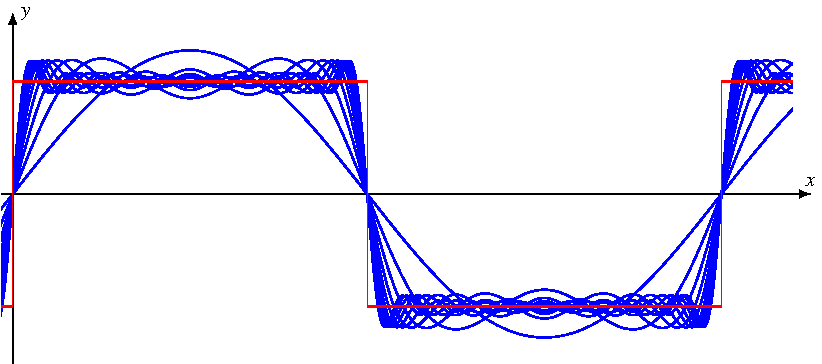
\includegraphics{chapters/010-skalarprodukt/images/fourierrechteck.pdf}
\caption{Approximation der Rechteckfunktion (rot) durch eine Folge
von Partialsummen der Fourier-Reihe.
\label{buch:skalarprodukt:fig:fourierrechteck}}
\end{figure}%
Die Supremum-Norm auf dem Raum der stetigen Funktionen hat den
Begriff der gleichmässig konvergenten Funktionenfolgen ergeben.
Cauchy-Folgen von stetigen Funktionen in der Supremum-Norm konvergieren
wieder gegen eine stetige Funktione.
Ist eine Funktion nicht stetig, lässt Sie sich im Sinne der Supremum-Norm
nicht durch stetige Funktionen approximieren.
Andererseits hat Fourier gezeigt, wie man technische wichtige Funktionen
wie die Rechteckfunktion durch trigonometrische Polynome
\begin{equation}
f_n(x)
=
\frac{4}{\pi} \sum_{k=0}^n \frac{\sin kx}{k}
=
\frac{4}{\pi} \biggl(
\sin x
+
\frac{\sin 3x}{3}
+
\frac{\sin 5x}{5}
+
\frac{\sin 7x}{7}
+
\ldots
\biggr)
\label{buch:skalarprodukt:eqn:rechteckreihe}
\end{equation}
approximieren kann.
Diese sind alle stetig und kommen der Rechteckfunktion in jedem Punkt,
in dem die Funktion stetig ist, beliebig nahe.
An den Stellen $x = n\pi$ hat die Grenzfunktion eine Sprungstelle,
die approximierenden Funktionen haben dort immer Abstand $1$
(siehe Abbildung~\ref{buch:skalarprodukt:fig:fourierrechteck}).
Die Folge ist also keine Cauchy-Folge und sie konvergiert nicht im
Sinne der Supremum-Norm.
Für solche Anwendungen muss eine besser geeignete Norm gefunden werden,
in der die Folge konvergiert.

%
% Skalarprodukt von Funktion
%
\subsubsection{Die $L^1$-Norm einer Funktion}
Die Supremum-Norm sieht nur den grössten Wert, die Konvergenz der Folge
\eqref{buch:skalarprodukt:eqn:rechteckreihe} ist aber nicht gleichmässig,
die maximale Abweichung ist immer $1$.
Gesucht ist eine Norm, die für die Folge
\eqref{buch:skalarprodukt:eqn:rechteckreihe} 
nur im Mittel eine Abweichung feststellt.
Für die Berechnung des Mittelwerts kann das Integral verwendet werden:

\begin{definition}
\label{buch:skalaprodukt:definition:l1norm}
Für eine stetige Funktion $X\to\mathbb{R}$, für die $x\mapsto |f(x)|$
integrierbar ist, heisst
\begin{equation}
\|f\|_1 = \int_X |f(x)|\,dx
\label{buch:skalarprodukt:eqn:l1norm}
\end{equation}
die {\em $L^1$-Norm} der Funktion $f$.
\end{definition}

Die $L^1$-Norm ist tatsächlich eine Norm, wir verifizieren die
definierenden Eigenschaften einer Norm.
\begin{enumerate}
\item
Definit: Sei $f$ eine stetige Funktion mit $\|f\|_1=0$
Wäre $f\ne 0$, dann gäbe es einen Punkt $x_0\in X$ mit $f(x_0) \ne 0$.
Da $f$ stetig ist, ist $f|(x)| > \frac12|f(x_0)|$ für $x$ in einer
$\delta$-Umgebung von $x_0$.
Dann folgt für die $L^1$-Norm
\begin{align*}
\|f\|_1
=
\int_X |f(x)|\,dx
\ge
\frac12 |f(x_0)| \cdot \delta 
> 0.
\end{align*}
Dies widerspricht der Annahme, dass $\|f\|_1=0$ ist, also muss $f=0$ sein.
\item
Homogeneität folgt durch direkte Rechnung
\[
\|\lambda f\|_1
=
\int_X |\lambda f(x)|\,dx
=
|\lambda|
\int_X |f(x)|\,dx
=
|\lambda| \cdot \|f\|.
\]
\item
Die Dreiecksungleichung folgt aus
\[
\|f+g\|_1
=
\int_X |f(x) + g(x)|\,dx
\le
\int_X |f(x)| + |g(x)|\,dx
=
\int_X |f(x)| + \int_X |g(x)|\,dx
=
\|f\|_1 + \|g\|_1.
\]
\end{enumerate}

Die $L^1$-Norm ist etwas ``schwächer'' als die Supremum-Norm im
folgenden Sinne.
Eine in der Supremum-Norm konvergente Funktionenfolge auf einem
kompakten Definitionsbereich $X$ ist auch in der $L^1$-Norm konvergent.
Zur Unterscheidung der verschiedenen Normen werden wir in Zukunft die
Supremum-Norm manchmal auch als $\|f\|_{\infty} = \|f\|$ schreiben.

\begin{satz}
Ist $X$ eine kompakte Teilmenge von $\mathbb{R}$ und $f_n$ eine
in der Supremum-Norm konvergente Folge stetiger Funktionen $f_n$,
dann ist $f_n$ auch in der $L^1$-Norm konvergent.
\end{satz}

\begin{proof}
Konvergenz in der Supremum-Norm bedeutet, dass für jedes $\varepsilon>0$
ein $N>0$ existiert derart, dass $|f_n(x)-f(x)|<\varepsilon$ für alle
$x\in X$ und alle $n>N$.
Für die $L^1$-Norm gilt dann
\begin{align*}
\|f_n-f\|_1
&=
\int_X |f_n(x) - f(x)|\,dx
\le
\int_X \varepsilon \,dx
=
\varepsilon \int_X \,dx
=
\varepsilon \operatorname{vol}(X).
\end{align*}
Da für einen kompakten Definitionsbereich $\operatorname{vol}(X)<\infty$
gilt, bedeutet dies, dass die $\|f_n-f\|_1\to 0$, dass also $f_n$ in
der $L^1$-Norm konvergiert.
\end{proof}

\begin{beispiel}
Die Folge $f_n(x)$ von \eqref{buch:skalarprodukt:fig:fourierrechteck}
konvergiert tatsächlich in der $L^1$-Norm auf dem Intervall $[0,2\pi]$.
Zwar ist $f_n$ nicht gleichmässig konvergent, aber fast.
Man kann zeigen, dass für jedes $\delta>0$, die Funktionen
$f_n(x)$ in Punkten $x$, die weiter als $\delta$ von den
Punkten $k\pi$ mit $k\in\mathbb{Z}$, gleichmässig konvergieren.
Innerhalb einer $\delta$-Umgebung der Vielfachen von $\pi$ ist die
$f_n(x)-f(x)$ beschränkt.
Die genaue Schranke ist nicht wichtig, wir nennen sie $M$ und bekommen
\[
|f_n(x)-f(x)|
\le M
\quad\forall x\in X.
\]
Ausserhalb einer kleinen Umgebung konvergiert die Folge gleichmässig,
zu jedem $\varepsilon>0$ gibt es also ein $N>0$ derart, dass
\[
|f_n(x)-f(x)|<\varepsilon
\]
für $x$ weiter als $\delta$ von $k\pi$ entfernt.
Für die $L^1$-Norm folgt dann
\begin{align*}
\|f_n-f\|_1
&=
\int_0^{2\pi} |f_n(x)-f(x)|\,dx
\\
&=
\int_0^\delta |f_n(x)-f(x)|\,dx
+
\int_\delta^{\pi-\delta} |f_n(x)-f(x)|\,dx
+
\int_{\pi-\delta}^{\pi+\delta} |f_n(x)-f(x)|\,dx
\\
&\qquad
+
\int_{\pi+\delta}^{2\pi-\delta} |f_n(x)-f(x)|\,dx
+
\int_{2\pi-\delta}^{2\pi} |f_n(x)-f(x)|\,dx
\\
&\le
\delta M
+
\varepsilon (\pi -2\delta)
+
2\delta M
+
\varepsilon (\pi -2\delta)
+
\delta M
\le
4\delta M + 2\pi\varepsilon
\end{align*}
für $n>N$.
Dadurch, dass man $\delta$ und $\varepsilon$ klein macht, kann man
also immer ein $N$ finden, so dass $\|f_n-f\|_1$ beliebig klein wird
für $n>N$.
Damit ist gezeigt, dass die Folge $f_n$ in der $L^1$-Norm konvergiert.
\end{beispiel}

Das Beispiel zeigt, dass die $L^1$-Norm eine schwäre Form der Konvergenz
ist, die eine erweiterte Klasse von Funktionen durch stetige Funktionen
zu approximieren erlaubt.

%
% Das $L^2$-Skalarprodukt
%
\subsubsection{Das $L^2$-Skalarprodukt}
Die $L^1$-Norm ist weniger strikt als die Supremum-Norm, aber sie ist
immer noch recht weit von der Intuition entfernt, die wir von der
Entfernungsmessung in der Geometrie haben, die von einem Skalarprodukt
herrühren.
Das Beispiel~\ref{buch:skalarprodukt:cauchyschwarz:beispiel:skalarprodukt}
weist den Weg, mit dem wir eine Norm für stetige Funktionen gewinnen
können, die von einem Skalarprodukt herkommt.

\begin{definition}
\label{buch:skalarprodukt:funktionraeume:definition:skalarprodukt}
Das {\em Skalarprodukt} stetiger Funktionen auf $X\subset \mathbb{R}$
ist definiert durch
\begin{equation}
\langle f,g\rangle
=
\int_X f(x)g(x)\,dx.
\label{buch:skalarprodukt:funktionraeume:eqn:skalarprodukt}
\end{equation}
\end{definition}

Es genügt nachzurechnen, dass $\langle f,g\rangle$ die Eigenschaften
eines Skalarproduktes hat, dann folgt die Dreiecksungleichung automatisch.
Zunächst ist klar,
dass~\eqref{buch:skalarprodukt:funktionraeume:eqn:skalarprodukt}
bilinear ist:
\begin{align*}
\langle \lambda f_1+\mu f_2,g\rangle
=
\int_X (\lambda f_1(x) + \mu f_2(x)) g(x)\,dx
&=
\lambda\int_Xf_1(x)g(x)\,dx + \mu\int_X f_2(x)g(x)\,dx
\\
&=
\lambda\langle f_1,g\rangle + \mu\langle f_2,g\rangle
\\
\langle f,\lambda g_1+\mu g_2\rangle
=
\int_X f(x)(\lambda g_1(x)+\mu g_2(x))\,dx
&=
\lambda\int_X f(x)g_1(x)\,dx + \mu\int_X f(x)g_2(x)\,dx
\\
&=
\lambda\langle f,g_1\rangle + \mu\langle f,g_2\rangle.
\end{align*}
Die Bilinearform ist aber auch positiv definit: Für eine stetige
Funktion $f(x)$ gilt
\[
\langle f,f\rangle
=
\int_X f(x)^2\,dx \ge 0.
\]
Da auch $f(x)^2$ eine stetige Funktion ist,
verschwindet das Integral genau dann, wenn $f(x)=0\;\forall x\in X$ ist.

Die zum Skalarprodukt gehörige Norm 
\[
\|f\|_2
=
\int_X |f(x)|^2\,dx
\]
heisst auch die {\em $L^2$-Norm}.

%
% Nicht kompakte Definitionsbereiche
%
\subsubsection{Nicht kompakter Definitionsbereich}
Für stetige Funktionen auf einem kompakten Definitionsbereich scheinen
die drei Normen $\|\;\cdot\;\|_\infty$, $\|\;\cdot\;\|_1$ und
$\|\;\cdot\;\|_2$ zu den gleichen Konvergenzbegriffen zu führen.
In diesem Abschnitt soll gezeigt werden, dass dies für nicht kompakte
Definitionsbereiche nicht mehr gilt.
Nicht einmal die Menge der Funktionen, die eine endliche Norm haben,
ist gleich.

\begin{beispiel}
Auf dem Definitionsbereich $X=(0,1]$ hat die Funktion
$f(x)=\log x$ endliche $L^1$-Norm aber unendliche Supremum-Norm.

\medskip
\noindent
Wegen $\lim_{x\to 0+}\log x = -\infty$ folgt $\|\log\|=\infty$.
Für die $L^1$-Norm folgt mit der Substitution $y=\log x$ und
$dy = dx/x$ oder $dx = e^y\,dy$
\begin{align*}
\|\log\|_1
&=
\int_0^1|\log x|\,dx
=
-\int_0^1\log x\,dx
=
-\int_{-\infty}^0 e^y\,dy
=
-\biggl[ e^y \biggr]_0^{-\infty}
=
1.
\end{align*}
Insbesondere ist die $L^1$-Norm beschränkt.
\end{beispiel}

\begin{beispiel}
Auf dem Definitionsbereich $X=[1,\infty)$ hat die Funktion
$f(x)=1/x$ endliche $L^2$-Norm aber unendlich $L^1$-Norm.

\medskip
\noindent
Die Integrale für die Normen ergeben:
\begin{align*}
\|f\|_1
&=
\int_1^\infty \frac{1}{x}\,dx
&
\|f\|_2^2
&=
\int_1^\infty \frac{1}{x^2}\,dx
\\
&=\biggl[\log x\biggr]_1^\infty
&
&=\biggl[-\frac{2}{x}\biggr]_1^\infty
\\
&=\infty
&
&=2.
\end{align*}
Insbesondere ist die $L^1$-Norm unbeschränkt, die $L^2$-Norm dagegen
beschränkt.
\end{beispiel}

\begin{satz}
Eine stetige Funktion auf einem beschränkten Definitionsbereich $X$
mit endlicher $L^2$-Norm hat auch endliche $L^1$-Norm.
\end{satz}

\begin{proof}[Beweis]
Aus der Cauchy-Schwarz-Ungleichung folgt
\begin{align*}
\int_X |f(x)|\,dx
&=
\langle |f|, 1\rangle
\le
\|f\|_2\cdot \|1\|_2.
\end{align*}
Nach Voraussetzung an die Funktion $f$ ist der erste Faktor beschränkt,
der zweite Faktor ist $\operatorname{vol}(X)$ und nach Voraussetzung
auch beschränkt.
\end{proof}

Die Beispiele zeigen, dass die Existenz der Normen selbst für stetige
Funktionen für nicht kompakten Definitionsbereich nicht garantiert ist.
Die Erweiterung auf nicht stetige Funktionen kann muss daher beschränkt
werden auf eine Klasse von Funktionen, für die die entsprechende Norm
existiert.
Das kann bedeuten, dass nicht alle stetigen Funktionen in Betracht 
kommen und dass neue Funktionen, die nicht stetig sind, als
Grenzwerte auftreten können.

%
% Grenzen des Riemann-Integrals
%
\subsection{Grenzen des Riemann-Integrals
\label{buch:skalarprodukt:funktionenraeume:subsection:grenzen-riemann}}
In den vorangegangenen Rechnungen sind wir immer vom Riemann-Integral
ausgegangen, welches man im Analysisunterricht als erstes kennenlernt.
Man zeigt dort, dass es für stetige Funktionen existiert und für
gleichmässig konvergente Folgen von Funktionen der Grenzwert des
Integrals mit dem Integral des Grenzwertes übereinstimmt:
\[
\int_X \lim_{n\to\infty} f_n(x)\,dx
=
\lim_{n\to\infty}
\int_X f_n(x)\,dx
\]
Der vorangegangene Abschnitt hat gezeigt, dass wir die Klasse der
Funktionen ausdehnen müssen auf Funktionen, die nicht stetig sind,
für die aber immer noch die $L^1$- oder die $L^2$-Norm existiert.
Hier zeigen sich die Schwächen des Riemann-Integrals.
In diesem Abschnitt soll an Beispielen gezeigt werden, was schief
gehen kann, und wie das Problem gelöst werden kann.

%
% Abzählbar viele Stetigkeitsstellen
%
\subsubsection{Abzählbar viele Unstetigkeitsstellen}
Wir konstruieren eine Funktionenfolge von Riemann-integrierbaren 
Funktionen, die alle das Integral $0$ haben, deren Grenzfunktion
aber nicht mehr Riemann-integrierbar ist.

Die rationalen Zahlen im Intervall $[0,1]$ sind abzählbar, d.~h.~es
gibt eine Folge $n\mapsto q_n\in[0,1]\cap\mathbb{Q}$, in der jede
rationale Zahl im Intervall vorkommt.
Aus der Folge $q_n$ konstruieren wir jetzt die Folge von Funktionen
\[
f_n(x)
=
\begin{cases} 
1&\qquad\text{$x$ ist einer der Werte $q_1,q_2,\ldots,q_n$}\\
0&\qquad\text{sonst}.
\end{cases}
\]
Die Funktion $f_n(x)$ ist also an genau $n$ Stellen von $0$ erschieden
und hat dort den Wert $1$.
Das Riemann-Integral ``sieht'' endlich viele Sprungstellen nicht,
die Funktionen $f_n$ sind also alle Riemann-integrierbar und haben
das Integral
\[
\int_0^1 f_n(x)\,dx=0.
\]
Insbesondere ist auch
\[
\lim_{n\to\infty}\int_0^1 f_n(x)\,dx = 0.
\]
Andererseits ist die Grenzfunktion
\begin{equation}
f(x)
=
\begin{cases}
1&\qquad\text{$x\in[0,1]\cap\mathbb{Q}$ ist rational}\\
0&\qquad\text{sonst, $x$ ist irrational.}
\end{cases}
\label{buch:skalarprodukt:funktionenraeume:eqn:ratfunk}
\end{equation}
Das Riemann-Integral der Funktion $f(x)$ existiert nicht.
Dazu müsste man ja für eine Unterteilung $0=x_0<x_1<\dots x_n=1$
die Riemann-Summen
\[
\overline{I}
=
\sum_{k=0}^{n-1}
(x_{k+1}-x_k) \sup_{x_k\le \xi \le x_{k+1}} f(\xi)
\qquad\text{und}\qquad
\underline{I}
=
\sum_{k=0}^{n-1}
(x_{k+1}-x_k) \inf_{x_k\le \xi \le x_{k+1}} f(\xi)
\]
berechnen, und sie müssten bei Verfeinerung der Unterteilung
gegeneinander konvergieren.
Aufgrund der Konstruktion der Funktion $f(x)$ ist aber
\[
\sup_{x_k\le \xi \le x_{k+1}} f(\xi) = 1
\qquad\text{und}\qquad
\inf_{x_k\le \xi \le x_{k+1}} f(\xi) = 0,
\]
sodass
$\overline{I}=1$ und $\underline{I}=0$ ist, ganz unabhängig von
der Unterteilung.

Der Riemannsche Integralbegriff muss also für die Zwecke der Approxmation
mit der $L^1$ oder $L^2$-Norm erweitert werden, so dass er sinnvoll mit
abzählbar vielen Unstetigkeitsstellen umgehenn kann.
Insbesondere sollte er als Integral der Funktion $f(x)$ 
von \eqref{buch:skalarprodukt:funktionenraeume:eqn:ratfunk}
den Wert $0$ liefern.

%
% Masse
%
\subsubsection{Masstheorie}
Gesucht wird also ein Integral, das für eine grössere Klasse von
Funktionen definiert ist und welches sich bezüglich Grenzwerten
besser verhält als das Riemann-Integral.
Das Integral ist nur dann nützlich, wenn es für viele Funktionen
die gleichen Werte ergibt.

Die einfachsten Funktionen, die wir integrieren wollen, sind die
{\em Indikatorfunktionen}, Funktionen, die durch eine Teilmenge
\index{Indikatorfunktion}
$A\subset X$ definiert sind durch
\[
1_A(x)
=
\begin{cases}
1&\qquad\text{für $x\in A$}\\
0&\qquad\text{sonst}.
\end{cases}
\]
Für ein Intervall der Länge $\lambda(A)$ ist
\[
\int_X 1_A(x)\,dx = \lambda(A).
\]
Für Mengen, die sich aus vielen Intervallen zusammensetzen, erwarten wir
die Summenformel
\[
A=\bigcup_{k=1}^\infty A_k,
\quad
A_k\cap A_j = \emptyset\;\forall k\ne j
\qquad\Rightarrow\qquad
\lambda(A) = \sum_{k=1}^\infty \lambda(A_k).
\]
Ausserdem sollte für eine Teilmenge $A\subset B$ der Inhalt der
Differenz $\lambda(A\setminus B)=\lambda(A)-\lambda(B)$ sein.

So entsteht eine Klasse von Mengen, denen sinnvoll ein Inhalt 
zugeordnet werden kann.
Solche Mengen heissen {\em messbar}.
Dazu gehören alle Intervalle, aber auch alle Differenzen und
abzählbaren Vereinigungen von Intervallen und messbaren Mengen
sind wieder messbar.
Die Klasse der messbaren Mengen ist also sehr gross.
Es braucht natürlich noch einiges an Arbeit, um zu zeigen, dass
eine widerspruchsfreie Definition der Funktion $\lambda(A)$
tatsächlich möglich ist, die jeder messbaren Menge einen
Inhalt zuordnet.
Eine solche Funktion heisst ein {\em Mass}, das aus der Intervalllänge
konstruierte Mass heisst auch das Lebesgue-Mass nach Henri Léon Lebesgue..
\index{Lebesgue-Mass}%
\index{Mass}%

Von besonderem Interesse sind Mengen, deren Inhalt $0$ ist.

\begin{definition}
\label{buch:skalarprodukt:funktionenraeume:definition:nullmenge}
Eine Nullmenge bezüglich des Masses $\lambda$ ist eine messbare
Menge $A$ mit Mass $\lambda(A)=0$.
\index{Nullmenge}
\end{definition}

Der Riemannsche Integralbegriff lässt bei der Bestimmung des Masses
nur endlich viele Intervalle zu. 
Die Menge $Q$ der rationalen Zahlen im Intervall $[0,1]$ ist abzählbar
unendlich.
In jeder beliebigen Umgebung einer reellen Zahl in $[0,1]$ findet man
rationale Zahlen in $Q$, eine Überdeckung der Menge der rationalen
Zahlen mit endlich vielen Intervallen enthält daher immer auch alle
reellen Zahlen, mit der möglichen Ausnahme von endlich vielen Zahlen.
Der Inhalt, den der Riemannsche Integralbegriff der Menge $Q$ zuordnen
muss, ist daher $1$.

Der neue Massbegriff erlaubt, die Menge mit abzählbar vielen messbaren
Mengen zu überdecken.
Sei $q_k$ eine Folge, die alle rationalen Zahlen in $Q$ durchläuft.
Zu jedem $k$ konstruieren wir das Intervall
\[
A_k = (q_k-\varepsilon2^{-k},q_k+\varepsilon2^{-k})
\]
mit Inhalt $\lambda(A_k) = 2\varepsilon2^{-k}$.
Es ist klar, dass die Intervalle $A_k$ die ganze Menge $Q$ überdecken,
also
\[
Q\subset \bigcup_{k=1}^\infty A_k.
\]
Der Inhalt der Menge $Q$ ist daher
\[
\lambda(Q)
\le
\sum_{k=1}^\infty \lambda(A_k)
=
\sum_{k=1}^\infty 2\varepsilon 2^{-k}
=
2\varepsilon
\sum_{k=1}^\infty 2^{-k}
=
2\varepsilon.
\]
Da $\varepsilon$ beliebig klein gewählt werden kann, folgt, dass
$\lambda(Q)=0$ sein muss.
Aus diesem Beispiel lässt sich erahnen, dass der Lebesguesche Massbegriff
mit Grenzwerten besser umgehen kann als der aus dem Riemannschen Integral
abgeleitete.

%
% Lebesgue-Integral
%
\subsubsection{Lebesgue-Integral}
Aus der Konstruktion eines Masses $\lambda$ kann jetzt die Konstruktion
eines Integrals an die Hand genommen werden.
Dazu werden Funktionen durch Stufenfunktionen approximiert, die
von der Form
\[
f(x) = \sum_{k=1}^\infty a_k 1_{A_k}(x)
\]
sind, wobei $A_k$ messbare Mengen sind.
Für solche Funktionen ist die naheliegende Definition des Integrals
\[
\int_X f(x)\,d\lambda(x)
=
\sum_{k=1}^\infty a_k \lambda(A_k).
\]
Der wesentliche Unterschied zur Riemannsschen Konstruktion ist,
dass nicht nur Intervalle zulässig sind sondern beliebige messbare Mengen.
Die Berechnung des Inhalts einer messbaren Mengen beinhaltet bereits
die Möglichkeit, Grenzwerte zu bilden.
Auch hier ist viel Arbeit notwendig um nachzuweisen, dass sich aus diesem
Ansatz ein widerspruchsfreier neuer Integralbegriff ergibt.
Das so konstruierte Integral heisst das {\em Lebesgue-Integral} und
\index{Lebesgue-Integral}%
wird zur Unterscheidung vom gewöhnlichen Riemannschen Integral und
wegen der Bedeutung des Masses $\lambda$, welches eine grosse Rolle
bei seiner Konstruktion spielt mit
\[
\int_X f(x) \,d\lambda(x)
\]
bezeichnet.

Beim Riemannschen Integral haben endliche Mengen und Mengen mit endlich
vielen Häufungspunkten Inhalt $0$.
Viele abzählbare Mengen haben dagegen positiven Inhalt.
Das Lebesguesche Mass gibt allen abzählbaren Mengen den Inhalt 0.

Unterscheiden sich zwei Funktionen $f$ und $g$ nur auf einer Nullmenge,
sagt man, sie seien {\em fast überall} gleich, geschrieben
\[
f(x) = g(x) \qquad \text{fast überall}.
\]
Zwei fast überall gleiche Funktionen haben das gleiche Integral, denn
\[
\int_X f(x)\,dx - \int_X g(x)\,dx
=
\int_X f(x)-g(x)\,dx
=
\int_X 0\,dx=0
\]
weil das Integral einer fast überall verschwindenden Funktion $0$ ist.

%
% Funktionsklassen
%
\subsubsection{Klassen von fast überall gleichen Funktionen}
Verwendet man die mit dem Lebesgque-Integral berechnete $L^1$- oder
$L^2$-Norm, dann können Funktionen nicht voneinander unterschieden werden,
die fast überall gleich sind.
Grenzwerte von Funktionenfolgen in der $L^1$- oder $L^2$-Norm sind
daher nur bis auf eine Nullmenge bestimmt.

\begin{definition}
Die Menge der Lebesgue-integrierbaren Funktionen auf dem Definitionsbereich
$X\subset\mathbb{R}$ wird mit
\[
\mathscr{L}^1(X)
=
\mathscr{L}^1_{\mathbb{R}}(X)
=
\left\{ f\colon X\to \mathbb{R}
\;\left|\;
\text{$f$ ist $\lambda$-integrierbar und $\int_X|f(x)|\,dx< \infty$}
\right.\right\}
\]
bezeichnet.
Entsprechend besteht $\mathscr{L}^2(X)$ aus den Funktionen $X\to \mathbb{R}$,
für die $|f(x)|^2$ integrierbar ist.
Sie heissen auch die {\em quadratintegrierbaren} Funktionen.
\end{definition}

Das Lebesgue-Integral kann Funktionen, die sich nur auf einer Nullmenge
verschieden sind, nicht unterscheiden. 
Daher ist es notwenig, solche Funktionen in Klassen zusammenzufassen:

\begin{definition}
Die Relation
\[
f\sim g
\qquad:\Leftrightarrow \qquad f(x) = g(x)\quad\text{fast überall}
\]
ist eine Äquivalenzrelation.
Die Menge der Äquivalenzklassen von Funktionen in $\mathscr{L}^1(X)$
bezüglich dieser Relation werden mit $L^1(X)$ bezeichnet, ebenso werden
die Äquivalenzklassen von $\mathscr{L}^2(X)$ bezüglich der Relation $\sim$
mit $L^2(X)$ bezeichnet.
\end{definition}

Mit den Funktionsklassen in $L^1(X)$ und $L^2(X)$ lässt sich genau
so rechnen, wie man es sicht gewohnt ist.
Für die Summe von Funktionen $f_1\sim f_2$ und $g_1\sim g_2$ gilt
\[
\left.
\begin{aligned}
f_1(x)&=f_2(x)&&\text{fast überall}\\
g_1(x)&=g_2(x)&&\text{fast überall}\\
\end{aligned}
\quad
\right\}
\qquad
\Rightarrow
\qquad
f_1(x)+g_1(x) = f_2(x)+g_2(x)\quad\text{fast überall},
\]
denn die Menge, auf der sich $f_1+f_2$ und $g_1+g_2$ unterscheiden
ist höchstens die Vereinigung der Mengen, auf denen sich $f_1$ und 
$f_2$ bzw.~$g_1$ und $g_2$ unterscheiden.
Die Vereinigung von Nullmengen ist aber wieder eine Nullmenge.

%
% Lebesgue-Integral
%
\subsubsection{Dominierte Konvergenz}
Die Entwicklung des Lebesgueschen Integrallbegriffs war motiviert
vom Wunsch, ein Integral zu erhalten, welches sich bezüglich
Konvergenz von Funktionenfolgen besser verhält.
Tatsächlich liefert die Theorie den folgenden zentralen Satz.

\begin{satz}[Dominierte Konvergenz]
\label{buch:skalarprodukt:satz:dominierte-konvergenz}
Sei $f_n$ eine auf dem Definitionsbereich $X$ punktweise konvergente
Folge Lebesgue-integrierbarer Funktionen mit Grenzfunktion 
\[
f(x) = \lim_{n\to \infty} f_n(x).
\]
Sei ausserdem $g$ eine Lebesgue-integrierbare Funktion mit
$|f_n(x)|<g(x)$ für alle $x\in X$.
Dann ist $f$ Lebesgue-integrierbar und es gilt
\[
\lim_{n\to\infty} \int_X f(x)\,d\lambda(x)
=
\int_X f(x)\,d\lambda(x)
\]
\end{satz}

Der Satz der dominierten Konvergenz von Lebesgue ersetzt also die
Bedingung der gleichmässigen Konvergenz, die beim Riemann-Integral
erfolgreich war, durch die viel schächere Bedingung, dass alle
Funktionen unterhalb einer gemeinsamen integrierbaren Funktion bleiben.
Dadurch wird verhindert, dass die Funktionen $f_n$ nach $\infty$
``ausbrechen'' kann und gegen eine Funktion konvergieren, die nicht
mehr integrierbar ist.


%
% Berechnung von Lebesgue-Integralen
%
\subsubsection{Berechnung von Lebesgue-Integralen}
Das Lebesque-Integral löst also die technischen Probleme, die das
Riemann-Integral manchmal bei Funktionenfolgen hat, die gegen ein
Grenzfunktion konvergieren, der man ein sinnvolles Integral im
Lebesgueschen Sinnen zuordnen kann.
Doch wie berechnet man ein Lebesgue-Integral?

Stetige Funktionen lassen sich beliebig genau durch Treppenfunktionen
approximieren.
Die Konvergenz des Lebesgue-Integrals für solche Funktionenfolgen
garantiert daher, dass das Lebesgue-Integral für stetige
Funktionen mit dem Riemann-Integral übereinstimmt.
Insbesondere braucht es keinen neuen Formalismus für die 
Berechnung von Integralen.
Auch für Funktionen, die an höchstens endlich vielen Stellen unstetig
sind, stimmt das Riemann-Integral mit dem Lebesgue-Integral überein.

Man soll sich daher das Lebesgue-Integral vor allem als eine 
Erweiterung des Integrals auf Funktionen vorstellen, die als Grenzwerte
von Folgen stetiger Funktionen im Sinne der $L^1$- oder der $L^2$-Norm
auftreten können.
Stetigkeit kann dabei verloren gehen, aber Konvergenzeigenschaften
wie die dominierte Konvergenz von
Satz~\ref{buch:skalarprodukt:satz:dominierte-konvergenz}
bleiben erhalten.



